% !TEX root = ../main.tex

\section{Fenomenología de las Asimetrías Azimutales en EAS}
\label{sec:fenomenologia}

La reconstrucción estándar de eventos se basa en el supuesto de que la densidad de partículas y especificamente de muones de una lluvia atmosférica extensa (EAS) presenta una simetría circular en el plano perpendicular a su eje de propagación en el plano de la lluvia. Sin embargo, esta hipótesis sólo es estrictamente válida para lluvias verticales. Para lluvias inclinadas, la simetría en el plano de la lluvia se rompe de manera sistemática, dando lugar a patrones en la densidad de muones que presentan una fuerte dependencia con el ángulo azimutal ($\phi$).

En este capítulo se describe el origen físico de esta asimetría, originada por la competencia entre la atenuación longitudinal de la cascada, efectos puramente cinemáticos de divergencia (geométricos) y el efecto del campo geomagnético terrestre, y se define el formalismo matemático utilizado para su parametrización armónica.

\subsection{El plano de la lluvia y la ruptura de simetría}
\label{subsec:simetria_ruptura}

Para estudiar la distribución espacial de las partículas, es imperativo distinguir entre el sistema de referencia topográfico y el sistema intrínseco de la cascada. Los detectores del Observatorio Pierre Auger se encuentran fijos sobre la superficie terrestre, definiendo el \textit{plano del suelo} (o \textit{ground plane}). Sin embargo, la física del desarrollo de la cascada posee simetría cilíndrica (en su aproximación de orden cero) respecto a su propio eje de propagación. El plano perpendicular a este eje es como se define el \textit{plano de la lluvia} (o \textit{shower plane}).

A lo largo de todo este trabajo, las coordenadas espaciales utilizadas para caracterizar la densidad de partículas —la distancia radial al núcleo ($r$) y el ángulo azimutal ($\phi$)— están estrictamente definidas sobre el plano de la lluvia. Para obtenerlas, las posiciones de las estaciones activadas en el terreno se proyectan geométricamente sobre este plano transversal al eje, tal como se esquematiza en la Figura \ref{fig:plano_lluvia}.

\begin{figure}[H]
	\centering
	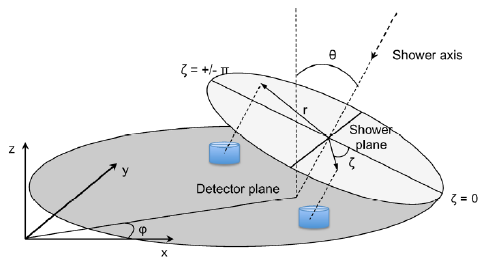
\includegraphics[width=0.7\textwidth]{capitulos/imagenes_capitulos/cap3/esquema_lluvia.png} 
	\caption{Esquema geométrico de una Lluvia Atmosférica Extensa (EAS). Se ilustra la proyección de las posiciones de los detectores desde el plano del suelo hacia el plano de la lluvia, definiendo las coordenadas intrínsecas $r$ y el ángulo azimutal $\phi$ (en el dibujo escrita como $\zeta$) del plano de la lluvia.}
	\label{fig:plano_lluvia}
\end{figure}

En el caso ideal de una lluvia estrictamente vertical ($\theta = 0^\circ$), ambos planos coinciden de manera exacta. En esta configuración, la distancia de vuelo que recorren las partículas desde el punto de primera interacción hasta alcanzar el nivel del suelo depende exclusivamente de la distancia radial al núcleo ($r$). Por lo tanto, los detectores ubicados a una misma distancia $r$ registrarán, en promedio, idénticas densidades de muones, reflejando una simetría circular perfecta e independiente del ángulo azimutal ($\phi$).


Sin embargo, cuando el rayo cósmico primario incide con un ángulo cenital $\theta > 0^\circ$, el plano de la lluvia deja de ser paralelo al plano del suelo. Esta inclinación geométrica rompe inherentemente la simetría del sistema respecto al observador terrestre.

Para comprender esta ruptura geométrica, es necesario analizar la intersección del frente plano de la lluvia con la superficie del arreglo. Al inclinar la cascada, los detectores ubicados a una misma distancia radial $r$ en el plano de la lluvia ya no se encuentran a la misma distancia física del máximo de desarrollo de la lluvia ($X_{max}$) y por ende las dinstintas particulas que componen la lluvia no atraviesan todas la misma cantidad de atomsfera antes de impactar contra el suelo. Esto define dos regiones azimutales extremas y fundamentales para el análisis de asimetrías:


\begin{itemize}
	\item \textbf{Región Temprana (\textit{Early}, $\phi \approx 0^\circ$):} Corresponde a la sección del frente de lluvia que se encuentra más cerca de la superficie topográfica y, por ende, impacta primero contra el arreglo de detectores. Las partículas que arriban a esta zona tienen el camino geométrico más corto y recorren la menor cantidad de atmósfera.
	\item \textbf{Región Tardía (\textit{Late}, $\phi \approx \pm 180^\circ$):} Corresponde a la sección diametralmente opuesta del frente, la cual se encuentra `elevada' respecto al suelo. Las partículas en esta dirección deben continuar propagándose a través de la atmósfera después de que el lado \textit{early} ya ha impactado, acumulando una distancia de vuelo significativamente mayor antes de ser detectadas y por ende siendo más atenuadas.
\end{itemize}

Esta diferencia estructural en las distancias de propagación para un mismo radio $r$ es el origen geométrico que cataliza los fenómenos físicos responsables de modular la densidad de muones, los cuales se describen a continuación.

\subsection{Origen físico de la modulación azimutal}
\label{subsec:origen_fisico}

La ruptura de la simetría circular no se debe a un único fenómeno, sino a la superposición de dos efectos principales que actúan en competencia directa y cuya dominancia depende de la distancia al eje de la lluvia.

\subsubsection{Atenuación atmosférica (dominancia \textit{early})}
\label{subsubsec:atenuacion}

El primer efecto es la atenuación atmosférica longitudinal. Las partículas que alcanzan la región tardía de la lluvia han atravesado una profundidad atmosférica considerablemente mayor que aquellas que impactan en la región temprana. Dado que la cascada evoluciona y se absorbe a medida que penetra en la atmósfera, este camino extra resulta en una mayor atenuación.

Este efecto genera un exceso aparente de densidad de partículas en la dirección $\phi = 0^\circ$ (\textit{early}) respecto a $\phi = \pm 180^\circ$ (\textit{late}). Si bien este mecanismo domina abrumadoramente la asimetría de la componente electromagnética en los detectores Cherenkov en agua (WCD), los muones, al tener un mayor poder de penetración y menor sección eficaz de interacción electromagnética, sufren una atenuación menor. No obstante, a grandes distancias del núcleo ($r > 400\text{ m}$), la atenuación atmosférica se vuelve el efecto dominante también para la componente muónica pura.

\subsubsection{Efectos geométricos y divergencia de ángulo sólido (dominancia \textit{late})}
\label{subsubsec:divergencia}

El segundo fenómeno subyacente es un efecto puramente cinemático y geométrico, producto de la divergencia de las partículas respecto al eje central de la lluvia. 

Para que una partícula alcance un detector ubicado a una distancia radial $r$ en la región temprana, debe ser emitida con un ángulo de divergencia grande respecto al eje de la cascada. Por el contrario, debido a la inclinación del frente, las partículas que impactan a la misma distancia radial $r$ en la región tardía requieren ángulos de divergencia mucho menores.

Dado que la densidad de partículas en una EAS está fuertemente concentrada cerca del eje (núcleo) y decae rápidamente conforme aumenta el ángulo de emisión, la región tardía logra muestrear una porción internamente más densa del haz primario. Este efecto geométrico induce un exceso de densidad de partículas en la región \textit{late} ($\phi = \pm 180^\circ$) que compite directamente con la atenuación atmosférica, dominando el comportamiento de la asimetría a distancias cercanas al núcleo ($r < 200\text{ m}$).

\subsection{Parametrización armónica de primer orden}
\label{subsec:parametrizacion}

Para cuantificar esta ruptura de simetría en la Función de Distribución Lateral (LDF), Billoir et al. \cite{Billoir2002} propusieron la inclusión de una parametrización de modulación cosinusoidal. Siguiendo este formalismo, la densidad de partículas (o la señal del detector) en el plano de la lluvia se modela como una función armónica de primer orden:

\begin{equation}
	S(r,\phi) = \langle S(r) \rangle \left( 1 + A_1(r, \theta) \cos\phi \right)
	\label{eq:asimetria_a1}
\end{equation}

donde $\langle S(r) \rangle$ es la densidad promedio a la distancia $r$ para una lluvia completamente simétrica, $A_1$ representa la amplitud de la asimetría temprano-tardía, y $\phi$ es el ángulo azimutal en el plano de la lluvia. Un valor de $A_1 > 0$ indica dominancia de la atenuación atmosférica (pico en la región \textit{early}), mientras que un $A_1 < 0$ señala la dominancia de efectos geométricos (pico en la región \textit{late}).

\subsection{Antecedentes en la Colaboración Auger}
\label{subsec:antecedentes}

Históricamente, el estudio de asimetrías azimutales en el Observatorio Pierre Auger se ha centrado en las señales medidas por el Detector de Superficie (SD). Los primeros estudios fenomenológicos como los de Pryke \cite{Pryke1998} y Billoir et al. \cite{Billoir2002} identificaron los patrones de asimetría en estaciones Cherenkov. Recientemente, con la actualización AugerPrime, Bradfield \cite{Bradfield2022} realizó análisis sistemáticos utilizando los detectores de superficie centelladores (SSD) combinados con los WCD, corroborando la utilidad de estas asimetrías para estudios de composición de masa.

Sin embargo, debido a que la señal del SD está invariablemente dominada por la componente electromagnética a los ángulos cenitales considerados, la magnitud intrínseca y la fenomenología de la asimetría temprano-tardía para una señal pura de muones duros ha permanecido inexplorada. Abordar este vacío utilizando las capacidades del UMD es el propósito central de los siguientes capítulos.
